%%%
% Plantilla de Memoria
% Modificación de una plantilla de Latex de Nicolas Diaz para adaptarla 
% al castellano y a las necesidades de escribir informática y matemáticas.
%
% Editada por: Mario Román
%
% License:
% CC BY-NC-SA 3.0 (http://creativecommons.org/licenses/by-nc-sa/3.0/)
%%%

%%%%%%%%%%%%%%%%%%%%%%%%%%%%%%%%%%%%%%%%%
% Thin Sectioned Essay
% LaTeX Template
% Version 1.0 (3/8/13)
%
% This template has been downloaded from:
% http://www.LaTeXTemplates.com
%
% Original Author:
% Nicolas Diaz (nsdiaz@uc.cl) with extensive modifications by:
% Vel (vel@latextemplates.com)
%
% License:
% CC BY-NC-SA 3.0 (http://creativecommons.org/licenses/by-nc-sa/3.0/)
%
%%%%%%%%%%%%%%%%%%%%%%%%%%%%%%%%%%%%%%%%%

%----------------------------------------------------------------------------------------
%	PAQUETES Y CONFIGURACIÓN DEL DOCUMENTO
%----------------------------------------------------------------------------------------

%%% Configuración del papel.
% microtype: Tipografía.
% mathpazo: Usa la fuente Palatino.
\documentclass[a4paper, 20pt]{article}
\usepackage[a4paper,margin=1in]{geometry}
\usepackage[protrusion=true,expansion=true]{microtype}
\usepackage{mathpazo}

% Indentación de párrafos para Palatino
\setlength{\parindent}{0pt}
  \parskip=8pt
\linespread{1.05} % Change line spacing here, Palatino benefits from a slight increase by default


%%% Castellano.
% noquoting: Permite uso de comillas no españolas.
% lcroman: Permite la enumeración con numerales romanos en minúscula.
% fontenc: Usa la fuente completa para que pueda copiarse correctamente del pdf.
\usepackage[spanish,es-noquoting,es-lcroman,es-tabla,,es-nodecimaldot]{babel}
\usepackage[utf8]{inputenc}
\usepackage{fontenc}
\selectlanguage{spanish}


%%% Gráficos
\usepackage{graphicx} % Required for including pictures
\usepackage{wrapfig} % Allows in-line images
\usepackage[usenames,dvipsnames]{color} % Coloring code
\graphicspath{{./fig/}}


%%% Matemáticas
\usepackage{amsmath}

%%% Pseudocódigo
\usepackage{algorithmicx}
\usepackage[ruled]{algorithm}
\usepackage{algpseudocode}

\newcommand{\alg}{\texttt{algorithmicx}}
\newcommand{\old}{\texttt{algorithmic}}
\newcommand{\euk}{Euclid}
\newcommand\ASTART{\bigskip\noindent\begin{minipage}[b]{0.5\linewidth}}
\newcommand\ACONTINUE{\end{minipage}\begin{minipage}[b]{0.5\linewidth}}
\newcommand\AENDSKIP{\end{minipage}\bigskip}
\newcommand\AEND{\end{minipage}}

%%% Código
\usepackage{listings}

%%% Tablas
\usepackage{tabularx}
\usepackage{float}
\usepackage{adjustbox}
\usepackage{booktabs}

% Enlaces y colores
\usepackage{hyperref}
\usepackage[dvipsnames]{xcolor}
\definecolor{webgreen}{rgb}{0,0.5,0}
\hypersetup{
  colorlinks=true,
  citecolor=RoyalBlue,
  urlcolor=RoyalBlue,
  linkcolor=RoyalBlue
}

%%% Bibliografía
\usepackage[backend=biber]{biblatex}
\DefineBibliographyStrings{spanish}{
  urlseen = {Último acceso}
}
\addbibresource{IN-P2.bib}

%----------------------------------------------------------------------------------------
%	TÍTULO
%----------------------------------------------------------------------------------------
% Configuraciones para el título.
% El título no debe editarse aquí.
\renewcommand{\maketitle}{
  \begin{flushright} % Right align
  
  {\LARGE\@title} % Increase the font size of the title
  
  \vspace{50pt} % Some vertical space between the title and author name
  
  {\large\@author} % Author name
  \\\@date % Date
  \vspace{40pt} % Some vertical space between the author block and abstract
  \end{flushright}
}

%% Título
\title{\textbf{Título}\\ % Title
Subtítulo} % Subtitle

\author{\textsc{Autor1,\\Autor2} % Author
\\{\textit{Universidad de Granada}}} % Institution

\date{\today} % Date

%-----------------------------------------------------------------------------------------
%	DOCUMENTO
%-----------------------------------------------------------------------------------------

\begin{document}

%-----------------------------------------------------------------------------------------
%	TITLE PAGE
%-----------------------------------------------------------------------------------------

\begin{titlepage} % Suppresses displaying the page number on the title page and the subsequent page counts as page 1
	
	\raggedleft % Right align the title page
	
	\rule{1pt}{\textheight} % Vertical line
	\hspace{0.05\textwidth} % Whitespace between the vertical line and title page text
	\parbox[b]{0.8\textwidth}{ % Paragraph box for holding the title page text, adjust the width to move the title page left or right on the page
		
		{\Huge\bfseries Práctica 2:\\[0.5\baselineskip] Análisis Relacional mediante\\ \\ Segmentación}\\[2\baselineskip] % Title
		{\large\textit{Curso 2019/2020}}\\[4\baselineskip] % Subtitle or further description
		{\Large\textsc{Sofía Almeida Bruno}\\[0.5\baselineskip]sofialmeida@correo.ugr.es} % Author name, lower case for consistent small caps
		
		\vspace{0.4\textheight} % Whitespace between the title block and the publisher
		
		{\noindent Grupo IN 2\\[0.5\baselineskip] Jueves 9:30-10:30}\\[\baselineskip] % Publisher and logo
	}

\end{titlepage}

%% Resumen (Descomentar para usarlo)
%\renewcommand{\abstractname}{Resumen} % Uncomment to change the name of the abstract to something else
%\begin{abstract}
% Resumen aquí
%\end{abstract}

%% Palabras clave
%\hspace*{3,6mm}\textit{Keywords:} lorem , ipsum , dolor , sit amet , lectus % Keywords
%\vspace{30pt} % Some vertical space between the abstract and first section


%% Índice
{\parskip=2pt
  \tableofcontents
}
\pagebreak

%%% Inicio del documento
%%%%%%%%%%%%%%%%%%%%%%%%%%%%%%%%%%%%%%%%%%%%%%%%%%%%%%%%%%%%%%%%%%%
%       DESCRIPCIÓN DEL PROBLEMA
%%%%%%%%%%%%%%%%%%%%%%%%%%%%%%%%%%%%%%%%%%%%%%%%%%%%%%%%%%%%%%%%%%%
\section{Introducción}

Tras estudiar, en la práctica anterior, algoritmos de clasificación para un problema de aprendizaje supervisado, pasamos ahora a un problema de aprendizaje no supervisado. Utilizaremos diferentes algoritmos de agrupamiento o clustering para realizar un análisis relacional.

En este caso partiremos de los microdatos publicados por el Instituto Nacional de Estadística (INE) en 2018 sobre la última encuesta de fecundidad. Elegiremos tres casos de estudio diferentes, en los que seleccionaremos las variables a estudiar (en general, de tipo categórico) y las variables sobre las que aplicar clustering (no tiene interés aplicarlo sobre el resto de variables ya que podrían no ser relevantes), compararemos distintos algoritmos y analizaremos los resultados obtenidos de forma comparada.

El conjunto original dispone de 14556 respuestas a la encuesta, con 463 variables sobre identificación, datos biográficos, hogar, vivienda, padres, relaciones de pareja actual e historia, hijos, embarazo actual y anteriores,\dots

En cada caso de estudio utilizaremos y compararemos varios algoritmos de agrupamiento, centrándonos en dos de ellos para hacer un análisis más profundo y tratando de mejorar sus resultados mediante el ajuste de sus parámetros. Los algoritmos elegidos y los parámetros con los que usarlo inicialmente son los siguientes:

\begin{itemize}
\item \textbf{K-Means}. Agrupa los ejemplos en tantos grupos como se le haya indicado. Parte de unos centros iniciales, asigna a cada ejemplo el cluster correspondiente al centro más cercano, recalcula los centros y vuelve al paso anterior. Este proceso se repite hasta que no haya más cambios en los clusters. Al estar basado en centroides generará clusters convexos. \texttt{n\_clusters = 5}.
\item \textbf{MeanShift}. Este algoritmo está basado en la densidad de las muestras. A partir de un radio fijado, determina un número de clusters y va desplazando sus centros hacia las regiones más densas. Es otro ejemplo de algoritmo basado en centroides, los clusters generados serán también convexos. Estima \texttt{bandwidth} por defecto.
\item \textbf{Birch}. Agrupa los objetos según se vayan recibiendo, es un algoritmo de clustering incremental. Crea un árbol con las características de los clusters guardando solo la información necesaria para poder determinarlos. Cada nodo tendrá un número de subclusters acotado por el factor de ramificación y un umbral que determina si un nuevo ejemplo está lo suficientemente cerca del cluster para pertenecer a él. Cuando llega un objeto, desciende por el árbol escogiendo en cada nodo el de características similares. Si no pertenece a ningún cluster y no se ha superado el factor de ramificación, se crea un nuevo subcluster, en caso contrario es absorbido por el cluster en cuestión. El último parámetro a fijar es el número de clusters con el que quedarnos finalmente. \texttt{branching\_factor=25}, \texttt{threshold=0.25}, \texttt{n\_clusters=5}.
\item \textbf{DBSCAN}. Es un algoritmo basado en densidad que no utiliza centroides, por lo que los grupos generados pueden tener diversas formas. Utiliza dos parámetros para definir la densidad: un valor $\varepsilon$ que determina cuándo un objeto es densamente alcanzable a partir de otro, un número mínimo de objetos por los que podemos alcanzar a otro para afirmar que pertenecen al mismo cluster. Generará en ocasiones un grupo etiquetado como ``-1'' que contiene a aquellos puntos que no pueden ser agrupados. \texttt{eps=0.2}\footnote{Se partió de un valor inicial $\varepsilon = 0.5$,  pero al ver que no conseguía buenos resultados en los casos a estudiar se disminuyó tratando de conseguir más variedad en los grupos.}, \texttt{min\_samples=5}.
\item \textbf{Ward}. Este método se distingue de los demás en que es jerárquico, es decir, genera una jerarquía que según el nivel de corte dará distintos agrupamientos. En este caso se ha elegido un algoritmo que en cada paso va agrupando dos clusters (inicialmente cada objeto es un cluster) de forma que el agrupamiento minimice la varianza (media de la distancia al cuadrado de cada elemento al centroide). Especificaremos como parámetro en qué nivel de la jerarquía nos quedamos. \texttt{n\_clusters=5}.
\end{itemize}

Para comparar los resultados y rendimiento de los diferentes algoritmos según distintos índices(?):
\begin{itemize}
\item \textbf{Tiempo}. Mediremos el tiempo que tarda cada algoritmo en agrupar el mismo conjunto de datos. Aunque no es el factor más importante en clustering, puede ser determinante para decantarnos por los algoritmos más rápidos entre aquellos que consigan resultados similares lo suficientemente buenos.
\item \textbf{Calinski-Harabasz}. Es una ratio entre la dispersión intracluster e intercluster para todos los clusters, donde la dispersión se mide como la suma de las distancias al cuadrado. Un valor alto indica que los grupos son densos y están bien separados.
\item \textbf{Silhouette}. Este coeficiente mide cómo de similares son los objetos de un mismo cluster comparado con los de otros clusters. Toma valores en el intervalo $[-1,1]$. Un valor cercano a 1 indica que los clusters están muy concentrados y distantes a los demás, uno cercano a 0 señala que los clusters están superpuestos y uno cercano a -1 que el agrupamiento es incorrecto.
\item \textbf{Número de clusters}. Comparando este valor observaremos si algún algoritmo no logra agrupar correctamente, por hacer demasiados clusters o, por el contrario, por no agrupar lo suficiente. En los algoritmos que sea un parámetro fijo podemos variarlo y ver cuál es el número de clusters que mejor se adapta a nuestro conjunto.
\end{itemize}

%%%%%%%%%%%%%%%%%%%%%%%%%%%%%%%%%%%%%%%%%%%%%%%%%%%%%%%%%%%%%%%%%%%
%       Caso de estudio 1 - PRIMER HIJO CON MÁS DE 30 AÑOS
%%%%%%%%%%%%%%%%%%%%%%%%%%%%%%%%%%%%%%%%%%%%%%%%%%%%%%%%%%%%%%%%%%%
\section{Caso de estudio 1 - Primer hijo con más de 30 años}
% Qué se analiza y por qué (indicar nº de datos que representa el caso de estudio)
En el resumen del INE sobre esta encuesta no se realizó un análisis de agrupamiento como el desarrollado en esta práctica, como mucho se relacionaron dos variables. Tomando como inspiración el resumen \cite{resINE} del INE, que muestra algunos resultados destacados obtenidos a partir de dicha encuesta, enfocaré el primer caso de estudio al retraso en la maternidad. Para ello, calculo (a partir de los datos dados) la edad media en la que las mujeres tienen su primer hijo: a los 24 años. Así, fijo como primer caso de estudio el conjunto de \textit{mujeres que tuvieron su primer hijo con 30 años o más}. Este subconjunto está formado por 1545 objetos.

Para realizar el agrupamiento en este conjunto selecciono cuatro variables que pueden ayudarnos a distinguir la situación y preocupaciones de las mujeres con una maternidad tardía:
\begin{itemize}
\item \textbf{NHIJOSDESEO} es el número de hijos que le gustaría o hubiera gustado tener a la entrevistada.
\item \textbf{ANORELACION} indica el año en el que comenzó la relación sentimental actual.
\item \textbf{ANOTRABACT} representa el año en el que la mujer comenzó a trabajar en su puesto actual.
\item \textbf{EDADIDEAL} como su nombre indica, es la edad que la entrevistada considera oportuna para tener el primer hijo.
\end{itemize}

Una vez fijado el caso de estudio y las variables mediante las que agrupar, utilizamos el \textit{script} \texttt{caso1.py} para ejecutar los cinco algoritmos y obtener tanto la tabla de resultados como los diferentes tipos de gráficos asociados. Podemos observar en la Tabla \ref{tab:algorithms1} los índices obtenidos en este caso de estudio.

% Tabla comparativa algotimos de clustering
\begin{table}[H]
\centering
\caption{Resultados caso de estudio 1}
\label{tab:algorithms1}
\begin{tabular}{lrrrr}
\toprule
Algoritmo & Tiempo ($s$) & Calinski-Harabasz & Silhouette & Número de clusters\\
\midrule
KMeans & 0.063 & 580.785 & 0.27533 & 5 \\
MeanShift & 9.857 & 9.770 & 0.32542 & 2 \\
Birch & 0.087 & 321.158 & 0.26552 & 5 \\
DBSCAN & 0.035 & 28.496 & 0.38585 & 2 \\
Ward & 0.099 & 501.202 & 0.29108 & 5 \\
\bottomrule
\end{tabular}
\end{table}

En una primera lectura detectamos que el tiempo de ejecución del algoritmo MeanShift es considerablemente mayor que el del resto de algoritmos. Esto se debe a que cuando lo ejecutamos, como no especificamos el valor de los parámetros, los calcula usando \texttt{sklearn.cluster.estimate\_bandwidth} que, como indica su documentación \cite{bandwidth}, tarda un tiempo cuadrático sobre el número de objetos. El tiempo de ejecución del resto de algoritmos es similar, siendo un poco menor el de KMeans y DBSCAN.

También destaca el bajo número de clusters generados por los algoritmos DBSCAN y MeanShift: 2. Esto quiere decir que formaron un único grupo (DBSCAN con el 98.83\% de los objetos, MeanShift con el 99.68\%) y juntó en el otro cluster, los objetos que no encajaban en él. Esto provoca que los objetos del cluster único estén muy separados de los del otro cluster, esta es la posible causa de que el índice Silhouette sea más elevado que en el resto de casos.

Para realizar un análisis de los grupos me centraré en los algoritmos KMeans y Birch.

\subsection{Análisis KMeans}

El algoritmo KMeans genera 5 grupos, como habíamos indicado, vemos en la Figura \ref{fig:KMeans_tam1} la distribución de los objetos en los distintos grupos.

\begin{figure}[H]
    \centering
    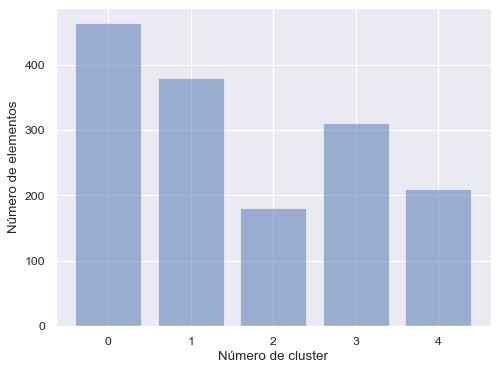
\includegraphics[width=0.6\textwidth]{./caso1/KMeans_tam_clusters}
    \caption{Caso 1 - Tamaño de los clusters- KMeans}
    \label{fig:KMeans_tam1}
\end{figure}

Los grupos tienen tamaños en rangos similares, entre 300 y 450 los tres mayoritarios, seguidos por un cluster con 209 elementos y el menor con 180. Para analizar los grupos, observamos en la Figura \ref{fig:KMeans_scatter1} la matriz de dispersión de las variables dos a dos y el histograma de cada una de ellas en la diagonal.

\begin{figure}[H]
    \centering
    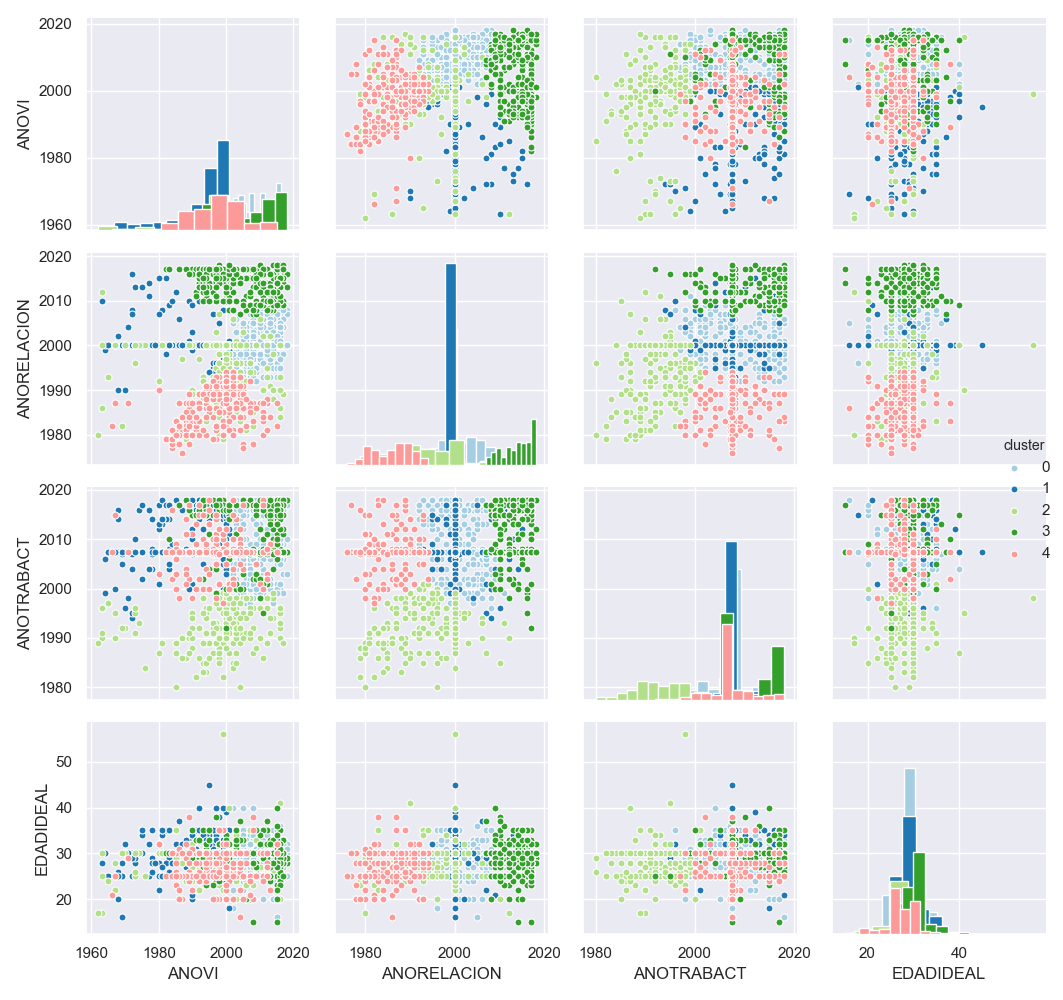
\includegraphics[width=1\textwidth]{./caso1/KMeans_scattermatrix}
    \caption{Caso 1 - Matriz de dispersión - KMeans}
    \label{fig:KMeans_scatter1}
\end{figure}

Las variables ANORELACION y ANOTRABACT sirven para separar bastante bien cuatro de los grupos, pero el resto también aporta información relevante. Aparentemente tenemos 4 grupos bien definidos y uno un poco más disperso, el cluster 1. Al cambiar el valor del parámetro \texttt{n\_clusters} descubriremos si al reagrupar se consiguen clusters más compactos. Rellenaremos la Tabla \ref{tab:carac_kmeans_1} con ayuda del diagrama de cajas mostrado en la Figura \ref{fig:KMeans_boxplot1} para hacernos una idea de las características principales de cada grupo.

\begin{figure}[H]
    \centering
    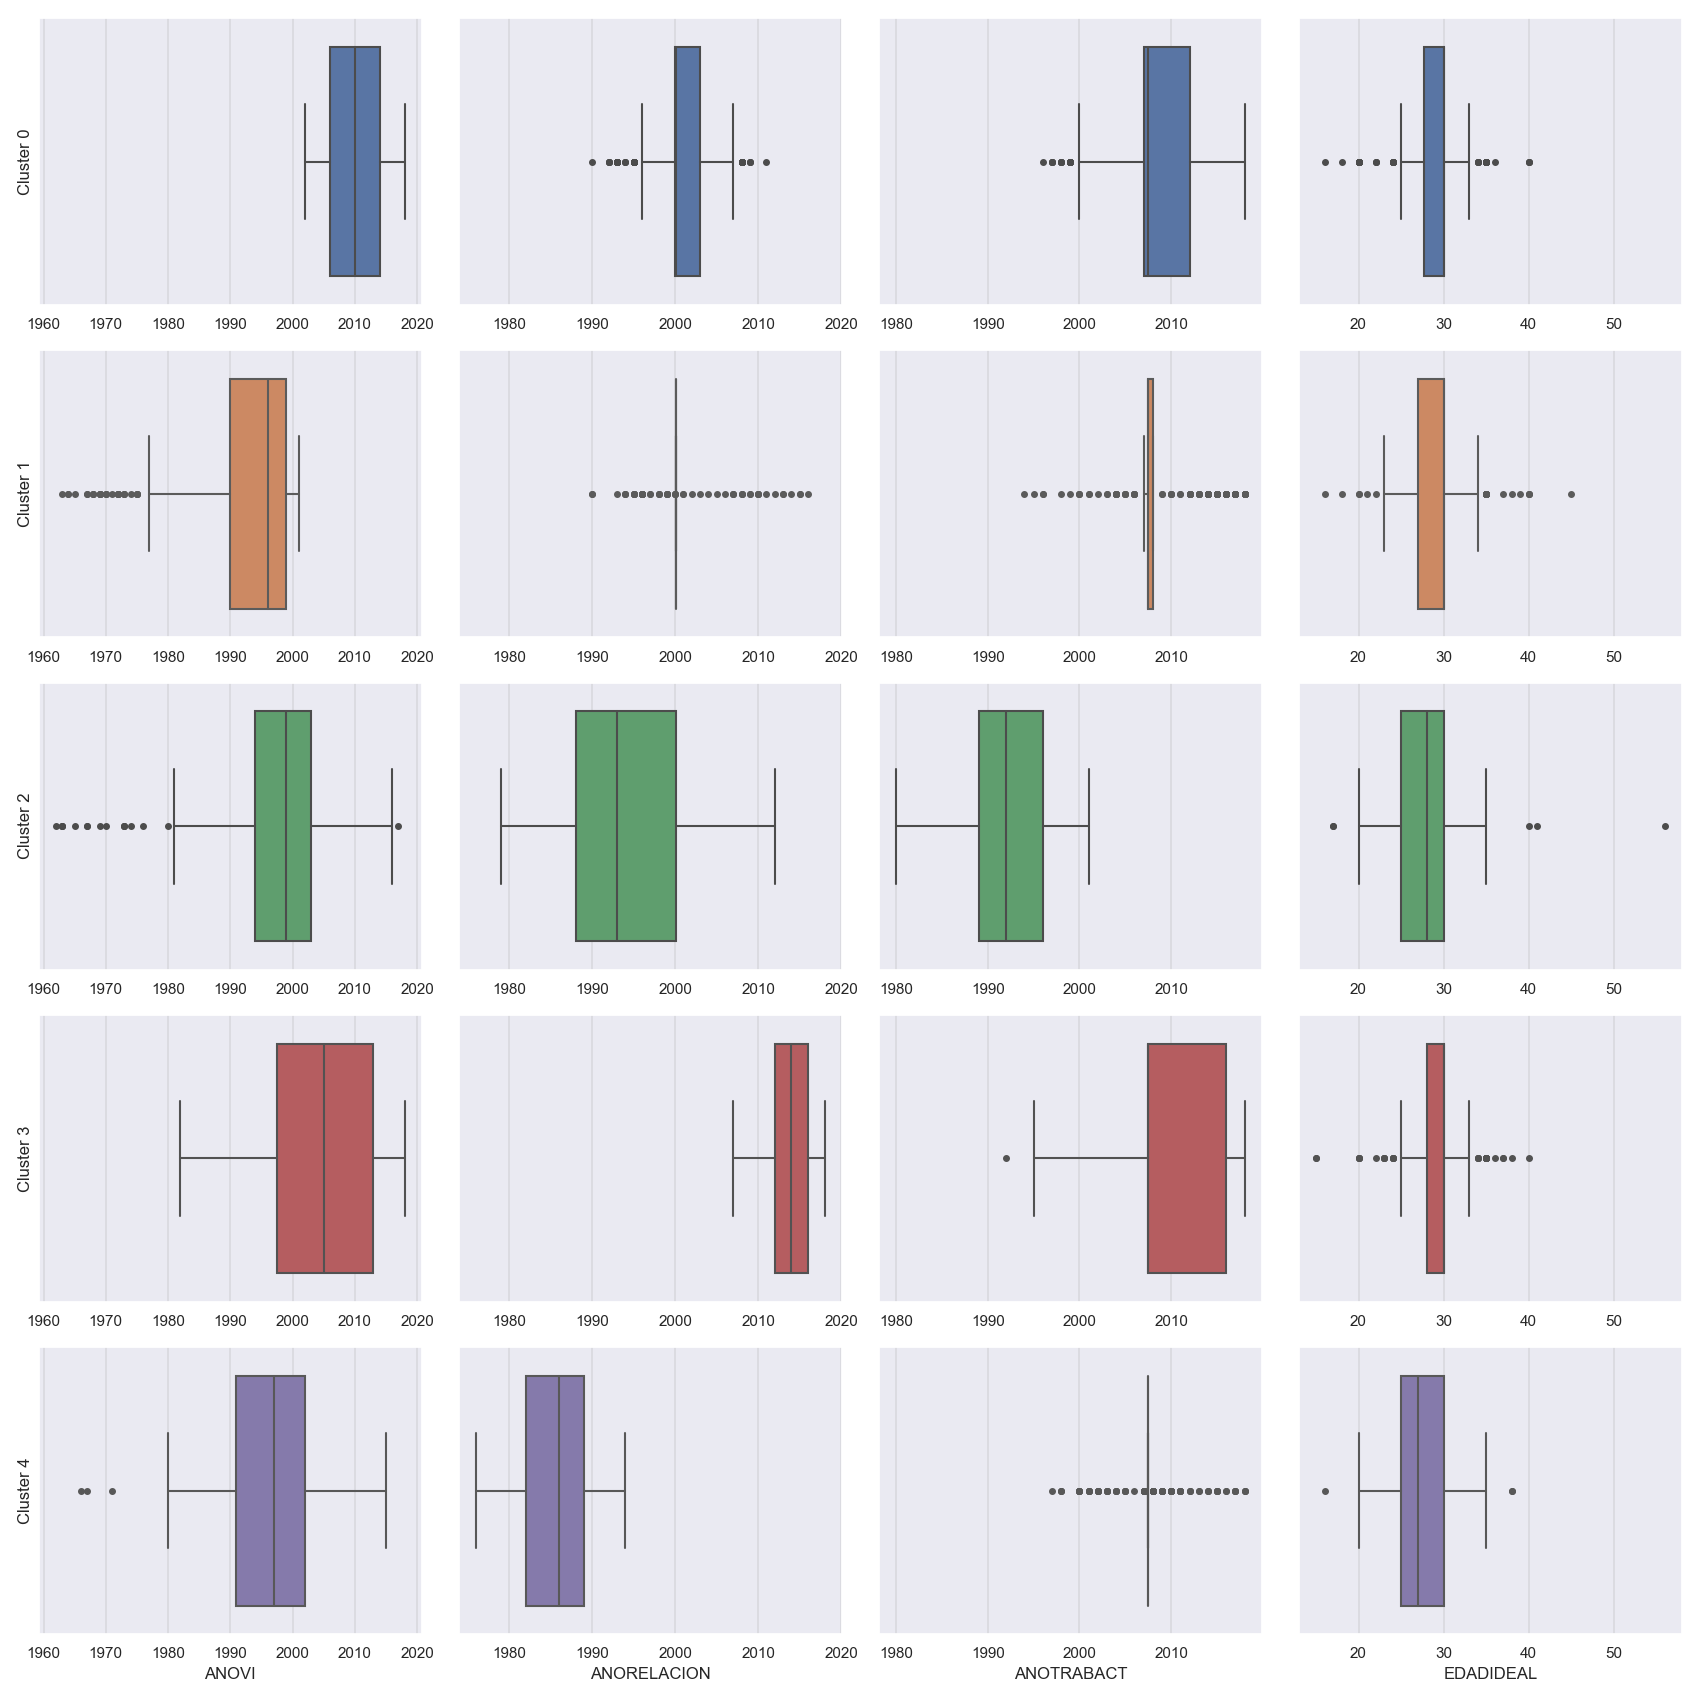
\includegraphics[width=1\textwidth]{./caso1/KMeans_boxplot}
    \caption{Caso 1 - Diagrama de cajas - KMeans}
    \label{fig:KMeans_boxplot1}
\end{figure}

% Tabla características de los grupos generados por KMeans
\begin{table}[H]
\centering
\caption{Caso 1 - Características de los grupos - KMeans}
\label{tab:carac_kmeans_1}
\begin{tabular}{lrrrr}
\toprule
Cluster & ANOVI & ANORELACION & ANOTRABACT & EDADIDEAL\\
\midrule
0 & 2005-2015 & 2000-2003 & 2007-2012 & 28-30 \\
1 & 1990-1999 & 2000 & 2008 & 27-30 \\
2 & 1995-2003 & 1987-2000 & 1988-1996 & 25-30 \\
3 & 1997-2012 & 2012-2016 & 2007-2016 & 28-30 \\
4 & 1991-2002 & 1983-1989 & 2008 & 25-30 \\
\bottomrule
\end{tabular}
\end{table}

Destaca que la mayor parte de las entrevistadas consideran que la edad ideal para tener un hijo es como mucho 30 años. Aunque en cada grupo el rango de edad que se considera apropiado para tener un hijo varía, considerando el mayor subconjunto, en general podemos afirmar que las mujeres que tuvieron el primer hijo con más de 30 años consideran que lo ideal habría sido tenerlo antes.

El cluster 0, mayoritario, está caracterizado por las mujeres que comenzaron su relación en torno al año 2000 y pasaron a vivir con su pareja a partir del año 2005. Al igual que las mujeres del cluster 3, comenzaron a trabajar en el puesto actual a partir del año 2007, posiblemente después de tener ese primer hijo. El cluster 3 es opuesto a este, está formado por aquellas mujeres que llevaban un tiempo viviendo con su pareja actual (comenzaron dicha convivencia en un rango que va desde 1997 hasta 2012) y empezaron la relación sentimental posteriormente.

La variable que más nos ayuda a distinguir el cluster 2 es ANOTRABACT, las mujeres de este grupo llevan trabajando desde el siglo anterior en el mismo empleo. Mientras que para diferenciar al cluster 4 es el año de comienzo de la relación el que nos dará la clave. Las mujeres de este cluster comenzaron su relación actual en la década de los 80.

El cluster 1, como ya habíamos observado en la matriz de dispersión, es un cluster más disperso, contiene \textit{outliers}, o valores anómalos, en todas las variables.

\subsubsection{Análisis de parámetros}

En este algoritmo el parámetro decisivo es el número de clusters. A priori, dado un conjunto de datos tan grande y sin conocimiento experto sobre el problema, es difícil acertar con el número de grupos en los que dividir el subconjunto. Podríamos aumentar este número enormemente para conseguir clusters muy compactos, el límite sería que cada objeto fuera su propio cluster, pero entonces no cumpliríamos los objetivos buscados: obtener información de los datos al agruparlos según una serie de variables.

Para probar con distintas opciones de este parámetro implementé el \textit{script} \texttt{caso1-kmeans}, donde se ejecuta el algoritmo KMeans variando el parámetro \texttt{n\_clusters} en el rango de enteros $[2,15]$. En la Tabla \ref{tab:param_kmeans1} vemos los resultados obtenidos para cada valor del parámetro.

% Tablas comparativas para el análisis de parámetros
\begin{table}[H]
\centering
\caption{Resultados cambio de parámetros KMeans}
\label{tab:param_kmeans1}
\begin{tabular}{lrrrr}
\toprule
Número de clusters & Tiempo ($s$) & Calinski-Harabasz & Silhouette &\\
\midrule
2 & 0.023 & 680.214 & 0.32456 \\
3 & 0.024 & 580.263 & 0.26207 \\
4 & 0.038 & 560.781 & 0.24693 \\
5 & 0.052 & 587.885 & 0.31232 \\
6 & 0.064 & 588.794 & 0.28092 \\
7 & 0.079 & 583.712 & 0.29898 \\
8 & 0.128 & 578.210 & 0.30893 \\
9 & 0.159 & 559.847 & 0.30801 \\
10 & 0.160 & 538.586 & 0.30408 \\
11 & 0.205 & 524.341 & 0.30575 \\
12 & 0.192 & 514.181 & 0.31093 \\
13 & 0.251 & 508.801 & 0.31454 \\
14 & 0.261 & 493.823 & 0.31312 \\
15 & 0.289 & 484.230 & 0.30280 \\
\bottomrule
\end{tabular}
\end{table}

Como es natural, al aumentar el número de clusters, aumentan los cálculos a realizar. Como para reasignar los clusters vamos comprobando si cada objeto pertenece al mismo, al aumentar el número de clusters, crece también el número de operaciones a realizar y con ello el tiempo de ejecución, como se refleja en la Tabla \ref{tab:param_kmeans1}.

Para simplificar la comparación del valor de los dos coeficientes en función del número de grupos se han realizado las gráficas lineales mostradas en la figura \ref{fig:param_kmeans1}

\begin{figure}[H]
    \centering
    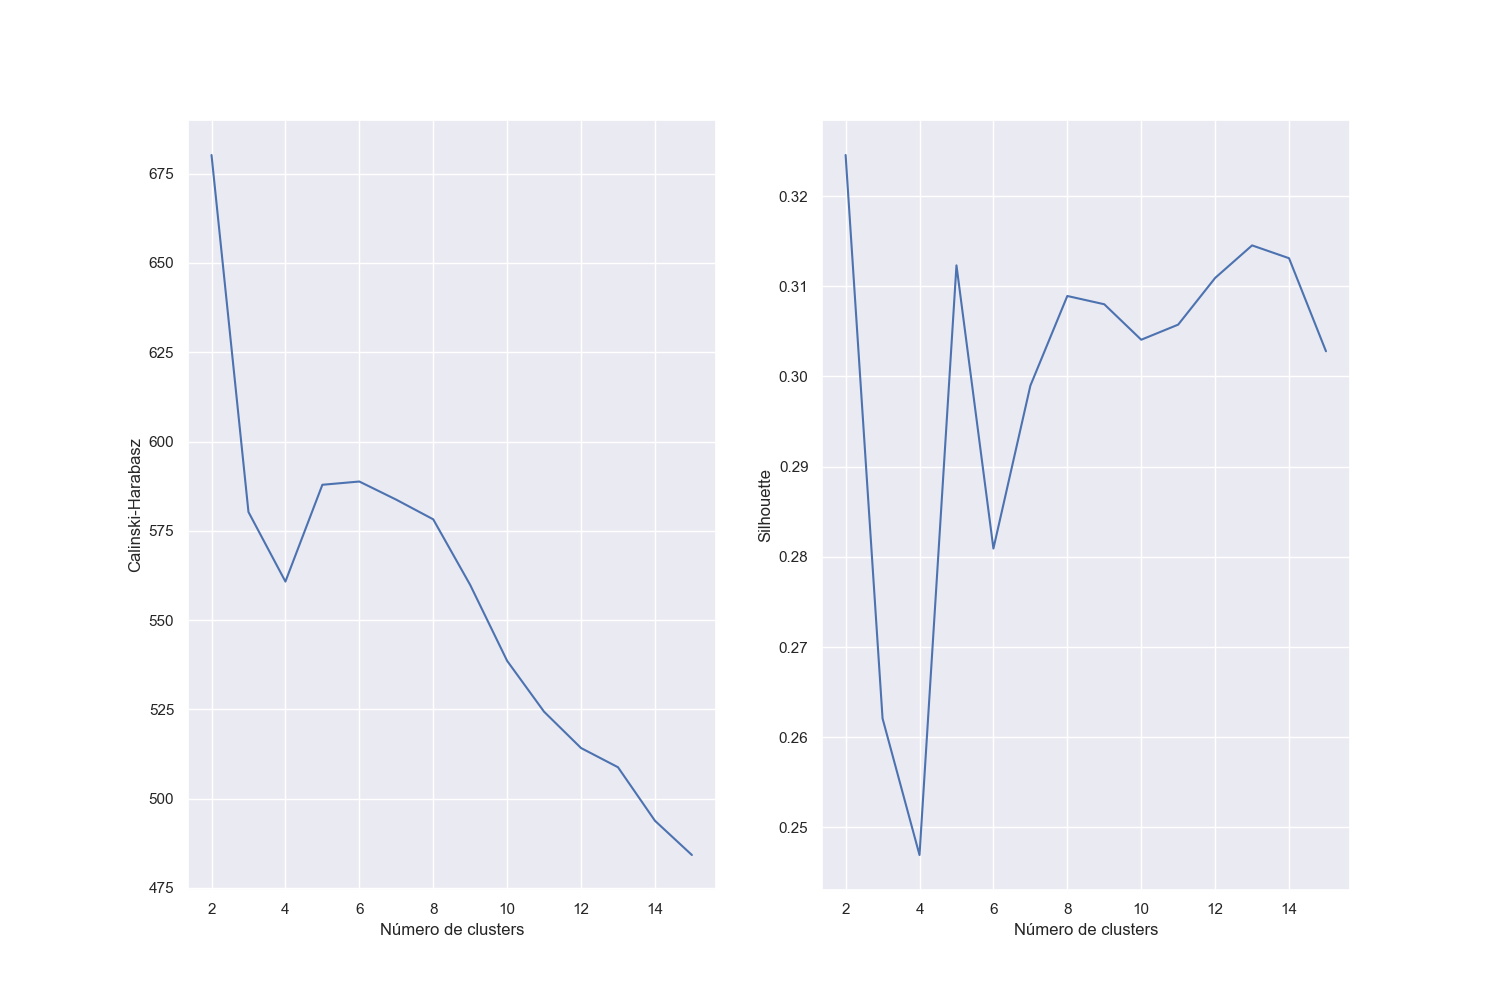
\includegraphics[width=1.2\textwidth, height=0.45\textheight]{./caso1/param_kmeans}
    \caption{Caso 1 - Comparación coeficientes según el número de clusters - KMeans}
    \label{fig:param_kmeans1}
\end{figure}

Para un número muy bajo de clusters, 2, ambos índices alcanzan sus valores máximos. Esto se debe a que al distinguir entre tan solo dos grupos es más fácil conseguir que los elementos queden cerca de su centro. Al ir aumentando el número de grupos, será más complicado diferenciar los elementos de la frontera, disminuyendo los coeficientes.

Observamos que ambos coeficientes alcanzan un máximo local en 5 clusters, nuestra estimación por defecto fue acertada.

El coeficiente Calinski-Harabasz disminuye a medida que aumenta el número de clusters pues aunque estén más concentrados, las diferencias entre ellos serán menores. Este hecho afecta más a este coeficiente que al coeficiente Silhouette, que a pesar de sufrir un mínimo local para 6 grupos aumenta y se mantiene en el rango $[0.30, 0.32]$ a partir de 8 clusters.

\subsection{Birch}


\subsection{Interpretación de la segmentación}
% Conclusiones generales

\newpage
%%%%%%%%%%%%%%%%%%%%%%%%%%%%%%%%%%%%%%%%%%%%%%%%%%%%%%%%%%%%%%%%%%%
%       REFERENCIAS
%%%%%%%%%%%%%%%%%%%%%%%%%%%%%%%%%%%%%%%%%%%%%%%%%%%%%%%%%%%%%%%%%%%
\printbibliography

%https://www.ine.es/dyngs/INEbase/es/operacion.htm?c=Estadistica_C&cid=1254736177006&menu=enlaces&idp=1254735573002 \label{ref:resINE}
%datos
%http://scikit-learn.org/stable/modules/clustering.html
%https://pythonspot.com/matplotlib-bar-chart/ -> Gráficos de tamaño de cluster
% https://matplotlib.org/3.1.1/tutorials/introductory/lifecycle.html -> same
% https://matplotlib.org/gallery/images_contours_and_fields/image_annotated_heatmap.html#sphx-glr-gallery-images-contours-and-fields-image-annotated-heatmap-py -> heatmap
%https://docs.w3cub.com/scikit_learn/auto_examples/cluster/plot_birch_vs_minibatchkmeans/ -> centros birch
\end{document}
